\vspace{-1cm}

\chapter{Grundlagen}
\label{cha:Grundlagen}

\vspace{-1cm}

\section{Regression}
\label{sec:Regression}

Regression beschreibt eine Methode, um die statistische Abhängigkeit zwischen Einflussvariablen und Zielvariable als mathematisches Modell zu beschreiben \parencite{RegressionGrundlagen}. Das Modell kann dabei als eine Funktion dargestellt werden. Diese Funktion nimmt Werte der Einflussvariablen an und gibt eine Vorhersage der Zielvariable\linebreak zurück. Dementsprechend kann das Modell ebenfalls verwendet werden, um den\linebreak Einfluss einzelner Variablen auf die Zielvariable zu analysieren.

% Aufgaben: Regression
% - Bessere Beischreibung für Regression
%   - Besser Quelle dafür finden -> Eventuell alternative zu einem Paper
%       - Eingehen auf Einfache Lineare Regression als quelle
%   - Genaue Unterscheidung zwischen Modell, Funktion
%   - Abgrenzung zu Machine-Learning Begriff

\noindent Eine bekannte Variante der Regression ist die einfache lineare Regression. Bei der\linebreak linearen Regression wird eine linearen Abhängigkeit zwischen Einflussvariablen und Zielvariable angenommen. Sie wird \emph{einfach} genannt, da sie nur eine einzelne Einflussvariable berücksichtigt. Dadurch sind die Ergebnisse des Modells einfach nachvollziehbar. Als ein Anwendungsbeispiel wird die einfach lineare Regression zur Analyse der\linebreak Bevölkerungsentwicklung\footnotemark  in Österreich verwendet. Als Einflussvariable wird die Jahreszahl verwendet. Die Zielvariable ist die Bevölkerung Österreichs für ein bestimmtes Jahr. Das Ergebnis des finalen Modells ist in Abbildung \ref{fig:pop_linear} ersichtlich.\\

\footnotetext{Datenquelle: STATcube - Statistische Datenbank von Statistik Austria \newline https://statcube.at/statistik.at/ext/statcube/jsf}

\begin{wrapfigure}{l}{0.55\textwidth}
\vspace{-1cm}
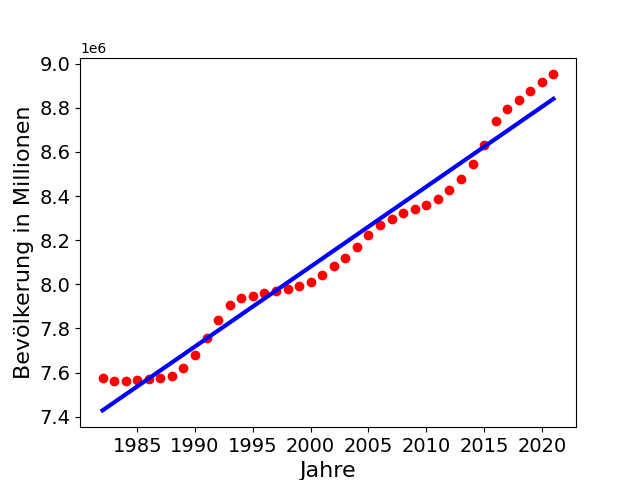
\includegraphics[width=0.6\textwidth]{images/population_linear.png}
\caption{Bevölkerungsentwicklung in Österreich}
\label{fig:pop_linear}
\vspace{-2.5cm}
\end{wrapfigure}

\noindent Die roten Punkte stellen die Ziel-\linebreak werte aus dem Datensatz dar. Die blaue Linie ist der Abbildung der Vorhersagen des Regressionsmodells. Die Visualisierung zeigt, dass das Modell das durchschnittliche Wachstum korrekt darstellt. Sie zeigt jedoch auch, das eine einfache lineare Regression keine genaue Vorhersage der Bevölkerung ermöglicht. Dafür ist eine andere Variante der Regression notwendig.

\vfill

\section{Visualisierung}
\label{sec:Visualisierung}

% Grundsätzliche Gründe für Visualisierung von Daten

Visualisierung stellt das Hauptthema dieser Bachelorarbeit dar. Einen guten Einstieg in dieses Thema bietet das Werk \emph{The visual display of quantitative information} \parencite{TufteEdward}. Demnach ist die Visualisierung ein Werkzeug zur Kommunikation von Daten. Die Stärke der Visualisierung ist es dabei, eine große Anzahl an Werten in einem kleineren Bereich darzustellen. Dadurch erleichtert die Visualisierung das Erkennen von Strukturen und Anomalien.\\
\noindent Diese Stärken sind im Vergleich der Abbildung  \ref{fig:visualization_advantage} zu sehen. Die Werte der Tabelle alleine sind nur schwer interpretierbar. Im Diagramm sind die Strukturen der beiden Klassen jedoch besser zu erkennen. Dort wird ersichtlich, dass sich die Punkte der beiden Klassen kaum überschneiden. Außerdem stechen in der Visualisierung die beiden Anomalien in den Daten heraus. Zwei Einträgen nähern sich dabei der jeweils anderen Klasse an. Die im Beispiel verwendeten Daten wurden mithilfe von Scikit-learn (Abschnitt \ref{sec:scikit-learn}) generiert.

\begin{figure}[H]
    \begin{minipage}{0.4\linewidth}
        \centering
        \begin{tabular}{ |c|c|c|c| } 
         \hline
           & X & Y & Klasse \\
          \hline
          0 & 1.771 & -1.54 & 1 \\
          1 & 4.346 & -7.57 & 1 \\
          2 & 5.737 & -9.69 & 1 \\
          3 & -1.07 & 1.486 & 0 \\
          4 & -1.37 & 1.528 & 0 \\
          5 & 1.342 & -8.97 & 1 \\
          6 & 1.417 & -9.93 & 1 \\
          7 & 1.336 & -1.34 & 1 \\
          8 & -5.78 & 2.561 & 0 \\
          9 & -1.21 & 1.173 & 0 \\
          \vdots & \vdots & \vdots & \vdots \\
          95 & -9.11 & 9.428 & 0 \\
          96 & -1.92 & 3.359 & 0 \\
          97 & -3.14 & 5.441 & 0 \\
          98 & 7.910 & -8.23 & 1 \\
          99 & -1.54 & 2.328 & 0 \\
         \hline
        \end{tabular}
    \end{minipage}
    \hfill
    \begin{minipage}{0.6\linewidth}
        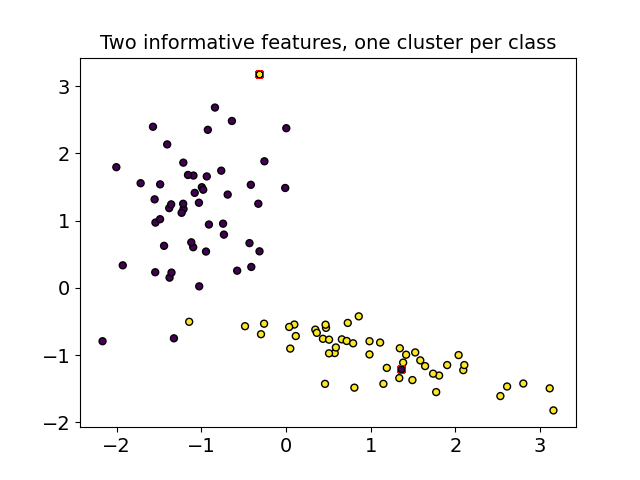
\includegraphics[width=1.1\linewidth]{images/visualization_advantage.png}
    \end{minipage}
    
    \caption{Beispiel zur Interpretation von Daten mittels Visualisierung}
    \label{fig:visualization_advantage}
\end{figure}

% Qualitätsmerkmale von Visualisierung und Warum sie wichtig sind
\noindent Für eine qualitative Visualisierung ist es wichtig die grafische Integrität einzuhalten. Laut Tufte wird dies durch das Einhalten von vier Regeln beschrieben:
\begin{enumerate}
    \item Konsistente Relation zwischen Größen in der Visualisierung und Zahlenwerten
    \item Konsistente Skalierung der Achsen
    \item Gleiche Anzahl an Dimensionen zwischen Visualisierung und Daten
    \item Darstellung aller für den Kontext relevanten Daten
\end{enumerate}

\noindent Diese Regeln wurden von Tufte in einem Zitat zusammengefasst: \emph{Show data variation, not design variation} \parencite{TufteEdward}. Das Brechen dieser Regeln, kann die Interpretation der dargestellten Daten beeinflussen.

% Aufgaben: Visualisierung
% - Beispiel für schlechte Umsetzung von Visualisierung / Visuelle Verzerrung


\section{Scikit-learn}
\label{sec:scikit-learn}

% Was ist scikit-learn?
Scikit-learn\footnote{https://scikit-learn.org/stable/index.html} \parencite{scikit-learn} ist eine Python-Bibliothek welche verschiedene Implementierungen von Machinelearning-Algorithmen bereitstellt. Ein Teil der Bibliothek stellt dabei verschiedene Implementierungen von Regression zur Verfügung. Ziel der\linebreak Bibliothek ist es, die Nutzung von Machinelearning-Algorithmen durch eine hohe Ebene der Abstraktion zu erleichtern. Zusätzlich bietet die Bibliothek eine gute Performance und eine umfassende Dokumentation der einzelnen Implementierungen. In der Praxis weist Scikit-learn eine weite Verbreitung vor. Das lässt sich aus den Statistiken der\linebreak Webseite \emph{libraries.io} feststellen\footnote{https://libraries.io/pypi/scikit-learn}. Dadurch ist die Unterstützung innerhalb von \linebreak Scikit-charts wichtig. Sie erlaubt es, dass Scikit-charts in vielen Projekten zur Anwendung kommen kann.\\\\
%Wie sieht die grundlegende API zur Verwendung aus?
\noindent Ein Überblick über die Schnittstellen der API ist in der Publikation \cite{sklearn_api} zu finden. Im Zentrum der Scikit-learn API befinden sich dabei drei Schnittstellen. Diese sind: \emph{estimator}, \emph{predictor} und \emph{transformer}.

\begin{itemize}
\item Der \emph{estimator} beschreibt ein Objekt, welches ein Modell aus Daten trainiert. Dafür wird eine \emph{fit} Methode definiert. Diese nimmt die Einflusswerte und optionale Zielwerte als Array an. Nach einem solchen Aufruf gilt das Modell als trainiert. Es kann nun für Vorhersagen und Analysen verwendet werden.
\item Der \emph{predictor} ist eine Erweiterung eines \emph{estimators}. Es beschreibt ein Objekt mit einer \emph{predict} Methode. Diese nimmt ein Array aus Einflusswerten entgegen und generiert daraus eine Vorhersage.
\item Der \emph{transformer} ist ebenfalls eine Erweiterung eines \emph{estimators}. Es beschreibt ein Objekt, welches Daten über eine \emph{transform}-Methode modifiziert oder filtert. Diese nimmt ein Array an und gibt die transformierte Version zurück.
\end{itemize}

\noindent Durch dieses flexible Design der API wird es ermöglicht, konkrete Implementierung auszutauschen. Dadurch wird es einfacher, allgemeine Algorithmen basierend auf diesen Modellen zu entwickeln. Im Rahmen dieser Arbeit ist besonders die \emph{predictor} Schnittstelle relevant. Diese bildet die Basis aller Regressionsmodell in Scikit-learn.

\section{Matplot}
\label{sec:matplot}

% Was ist Matplot und warum ist es interessant?
% Unterstützt 2D plots, 3D plots sowie interaktive Visualisierungen
% Hohe customizabilitie, viel einstellbar
% Wird in vielen Bibliotheken wie z.B. skicit-learn zur visualisierung verwendet
Bei Matplotlib \parencite{Matplot} handelt es sich um eine Python-Bibliothek zur Entwicklung von Visualisierungen. Die Bibliothek ermöglicht dabei sowohl 2D, 3D und\linebreak interaktive Visualisierungen. Die Visualisierungen können durch den Entwickler bis ins kleinste Detail konfiguriert werden. Dadurch werden auch komplexe Visualisierungen ermöglicht. Ein Beispiel dafür ist Abbildung \ref{fig:matplot_fig_anatomy}, welche mithilfe von Matplot generiert wurde. Die Abbildung dient ebenfalls als eine Übersicht über alle konfigurierbaren Elemente einer Visualisierung.

\begin{figure}[H]
\centering
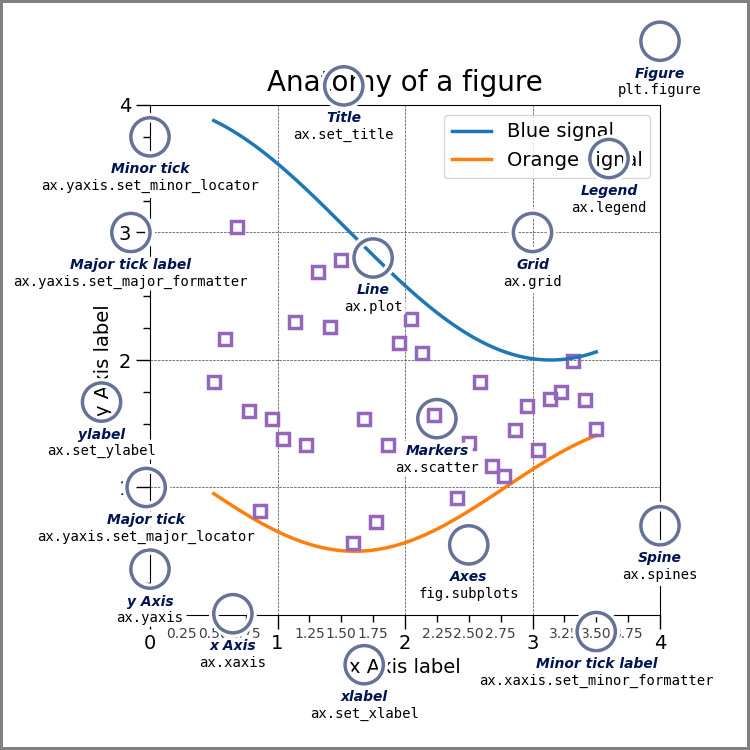
\includegraphics[width=.7\textwidth]{images/matplot_figure_anatomy.jpg}
\caption{Aufbau einer Matplotlib Visualisierung \protect\footnotemark}
\label{fig:matplot_fig_anatomy}
\end{figure}

\footnotetext{Quelle: https://matplotlib.org/3.7.1/gallery/showcase/anatomy.html}

% Wie sind die Klassen für das Rendering aufgebaut?
\noindent Basis einer Visualisierungen in Matplot sind laut API-Referenz\footnote{https://matplotlib.org/3.7.1/api/index.html} zwei Klassen: \emph{Figure} und \emph{Axes}. Eine \emph{Figure} beinhaltet alle Daten und Objekte einer Visualisierung. Diese kann einen übergreifende Titel, Legende, mehrere \emph{Axes} sowie \emph{Sub-Figures} beinhalten.\\
\noindent Eine \emph{Axes} beschreibt Bereiche einer \emph{Figure}, in welchen Daten dargestellt werden. Diese Objekte verwalten die einzelnen Linien, Datenpunkte sowie Achsenkonfigurationen. In der Abbildung \ref{fig:matplot_fig_anatomy} betrifft das alle hervorgehobenen Elemente, welche mit \emph{ax.} beginnen.\\\\
% Arten der Anwendung der API?
\noindent Die Anwendung der Matplot-API kann entweder explizit oder implizit erfolgen. Bei der expliziten Anwendung werden \emph{Figure}- und \emph{Axes}-Objekte direkt erstellt und verwaltet. Es handelt sich dabei um einen objektorientierten Ansatz. Bei der impliziten Anwendung wird die \emph{matplotlib.pyplot} API verwendet. Es handelt sich dabei um einen state-basierten Ansatz, bei welchem die Objekte von der API verwaltet werden. Für diese Arbeit wird rein die explizite Anwendung verwendet, um eine genaue Kontrolle über die Visualisierungen zu behalten.\\\\
% wo ist rendering unterstützt?
\noindent Um unterschiedliche Anwendungsfälle zu ermöglichen, unterstützt Matplot eine Reihe an \emph{Back-Ends} für die Darstellung. Nicht-interaktive Back-Ends werden zum Speichern von Visualisierungen verwendet (z.B. PNG, PDF, ...). Interaktive Back-Ends\linebreak unterstützen verschiedene betriebssystemunabhängige UI-Systeme, sowie einen Web-Server und \nameref{sec:jupyter_notebook}. Für diese Arbeit ist es dementsprechend notwendig zu Testen, ob die Diagramme auf den unterstützten \emph{Back-Ends} funktionieren. Gefundene Einschränkungen müssen ebenfalls hervorgehoben werden.

\section{Jupyter Notebook}
\label{sec:jupyter_notebook}

Jupyter Notebooks \parencite{kluyver2016JupyterN} sind ein Datenformat zum Austausch von Code-Ausschnitten und Beschreibungen. Über eine eigene Laufzeitumgebung\footnote{https://jupyter.org/} können die Notebooks interaktiv im Browser ausgeführt werden. Sie sind werden oft im\linebreak wissenschaftlichen Umfeld verwendet, um Ergebnisse auszutauschen. Sie besitzen ebenfalls eine Unterstützung der Programmiersprache Python. Für Scikit-charts ist es dementsprechend notwendig, Jupyter Notebooks zu unterstützen.

\section{ROC- / REC-Kurven}
\label{sec:roc_rec}

ROC und REC Kurven werden in einigen Bibliotheken zur Visualisierung von Regressionsmodellen angeboten. \emph{Receiver Operating Characteristic} (ROC) Kurven werden Verwendet, um die Qualität von Klassifizierungsfunktionen zu bewerten. Auf der Y-Achse wird dabei der Prozentsatz der echt positiven Werte aufgetragen. Auf der X-Achse wird der Prozentsatz der falsch positiven Werte aufgetragen. Die Performance wird bei ROC-Kurven in dem Bereich unter der Kurve (AUC) beschrieben. Diese ist bei zufälligen Funktionen etwa 0.5 und bei Funktionen mit immer richtigen Ergebnissen 1. Dieses Prinzip kann auch zum Vergleich zweier beliebiger Funktionen über ihre Ergebnisse angewandt werden.

\begin{wrapfigure}{l}{0.55\textwidth}
\vspace{-1cm}
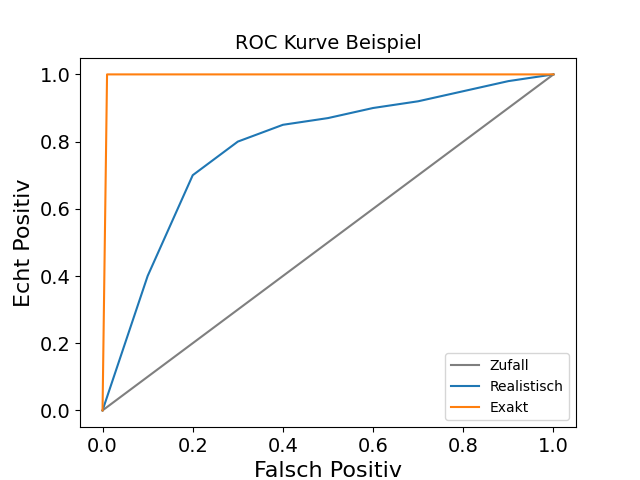
\includegraphics[width=0.6\textwidth]{images/roc_example.png}
\caption{Beispiel für ROC-Kurven}
\label{fig:roc_example}
\vspace{-4cm}
\end{wrapfigure}

\noindent Die \emph{Regression Error Characteristic} (REC) Kurve ist eine Anwendung des Prinzips von ROC für Regression. Im Gegensatz zur ROC-Kurve wird hier auf der X-Achse der absolute Unterschied zwischen Vorhersage und Zielwert dargestellt.\linebreak \parencite{RocRec}

\vspace{3.5cm}

\pagebreak

\section{Pandas}
\label{sec:pandas}

% Was ist es?
% Wie / wofür wird es verwwendet?
Pandas \parencite{pandas} ist eine Python-Bibliothek zur Verwaltung und Analyse von tabellarischen Daten. Sie wird in der Bibliothek zur Verwaltung der Diagrammdaten, sowie dem Laden des Beispieldatensatzes verwendet. Den Kern der\linebreak Bibliothek stellt die \emph{Dataframe} Datenstruktur. Diese verwaltet die Daten als eine\linebreak Tabelle. Der Zugriff auf die Daten ist beliebig über die Spaltennamen oder Zeilen-Indices möglich. Ein Zugriff kann ebenfalls mithilfe von Pythons \emph{Slicing}\footnote{https://docs.python.org/3/reference/expressions.html\#slicings} erfolgen. Dadurch ist es möglich, einzelne Teilbereiche als eigenen Dataframe auszuwählen.\\\\
\noindent Neben dem intuitiven Zugriff vereinfacht die Bibliothek das Serialisieren und Deserialisieren von Datensätzen. Dafür werden \emph{read\_} und \emph{write\_} Funktionen zur Verfügung\linebreak gestellt. Diese Unterstützen verschiedene Datenformate wie CSV, Excel, SQL oder JSON. Die Datenstruktur bietet außerdem eingebaute Funktionen zur Analyse der\linebreak Daten. Mithilfe dieser können beispielsweise Median, Durchschnittswert sowie Mininum und Maximum ausgewählt werden. Außerdem gibt es eine eingebaute Visualisierung der Daten mithilfe von Matplotlib. Beispielsweise können Histogramme, Boxplots oder Streudiagramme über die Daten generiert werden.



\section{Partial dependence}
\label{sec:partial_dependence}

Mithilfe der \emph{partial dependence}, zu deutsch \emph{partielle Abhängigkeit}, kann der relative Einfluss von Variablen auf eine Funktion beschrieben werden. Die partial dependence wird deshalb für die Darstellung des Schnittdiagramms benötigt. Wie dieser Wert berechnet wird ist in dem Buch "The Elements of
Statistical Learning" \parencite{elements_statistical_learning}\linebreak beschrieben.\\\\
\noindent Darin werden zwei Mengen $X_S$ und $X_C$ definiert. $X_S$ beschreibt die Einflussvariablen, für welche die partial dependence berechnet wird. $X_C$ beschreibt die restlichen Einflussvariablen. Das Ergebnis der Funktion $f(X)$ ergibt sich dementsprechend aus $f(X) = f(X_S, X_C)$. Das Ergebnis der Funktion für konkrete Werte von $X_S$ kann\linebreak somit durch den Erwartungswert über alle Werte von $X_C$ beschrieben werden. In der Bibliothek kann dies über die konkreten Werte $x_C$ im Datensatz angenähert werden.

\begin{equation}
  \begin{aligned}
    \bar{f}_S(X_S) = \frac{1}{N}\sum_{i=1}^{N}f(X_S, x_{iC})
  \end{aligned}
  \label{fig:partial_dependence}
\end{equation}

\noindent Der Wert $N$ entspricht dabei der Anzahl an Einträgen im Datensatz. Der Einfluss der Variablen $Xs$ wird beschrieben über die Relation zwischen den eingesetzten Werten sowie den Ergebnissen $\bar{f}_S(X_S)$.

%   - Partial-Dependency-Plot
%       - https://slds-lmu.github.io/iml_methods_limitations/pdp.html
%       - https://www.tandfonline.com/doi/full/10.1080/10618600.2014.907095
%       - https://en.wikipedia.org/wiki/Partial_derivative
%       - https://hastie.su.domains/ElemStatLearn/printings/ESLII_print12_toc.pdf Seite 388